\documentclass[addpoints]{exam}
\usepackage{amsmath}
\usepackage{amsfonts}
\usepackage[most]{tcolorbox}
\usepackage{tikz}
\usepackage{pgfplots}
\usepackage{mdframed}
\usepackage{hyperref}

\marksnotpoints
\pointsinrightmargin
\bracketedpoints

\hypersetup{
  colorlinks=true,
  linkcolor=blue,
  filecolor=magenta,
  urlcolor=blue,
  pdfpagemode=FullScreen,
}

\urlstyle{same}

\pagestyle{headandfoot}
\firstpageheadrule
\runningheadrule
\firstpageheader{Pre Calc Prep}{Functions}{Shah}
\runningheader{}{Functions}{}
\firstpagefooter{}{}{}
\runningfooter{ }{\thepage}{ }

\begin{document}

  \begin{tcolorbox}[breakable, title=QUADRATIC FUNCTIONS, colframe=black, sharp corners, colback=white, colbacktitle=white, coltitle=black]
    \Large \textbf{Introduction}
    \newline \normalsize
    As you are already familiar with, quadratic functions are functions in the form $ax^2+bx+c$. 
    When talking about quadratic functions the two main things we are looking at is the \textbf{vertx} and the \textbf{roots/zeros}.

    \vspace{0.3in}

    \begin{minipage}{0.45\linewidth}
      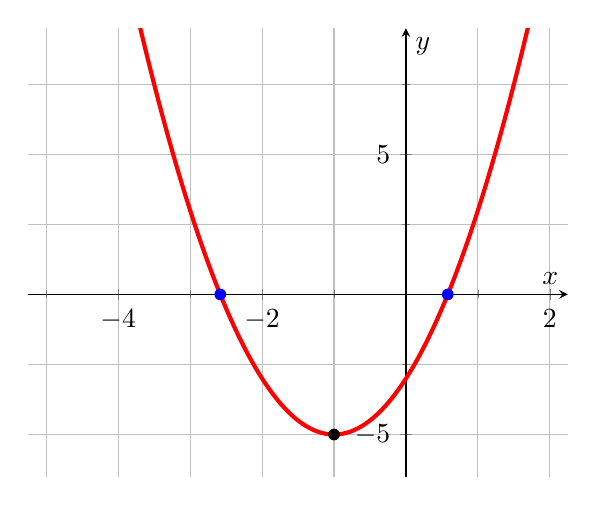
\begin{tikzpicture}
        \begin{axis}[
          grid=both,
          axis lines=center,
          xlabel={$x$},
          ylabel={$y$},
          minor tick num=1,
          xmin=-5.25,
          xmax=2.25,
          ymin=-6.5,
          ymax=9.5,
        ]

        \addplot[red, line width=1.5pt, samples=200]{2*x^2+4*x-3};

        \node[circle, fill, inner sep=1.5pt] at (axis cs: -1, -5){};
        \node[circle, blue, fill, inner sep=1.5pt] at (axis cs: 0.581, 0){};
        \node[circle, blue, fill, inner sep=1.5pt] at (axis cs: -2.581, 0){};

        \end{axis}
      \end{tikzpicture}
    \end{minipage}
    \hfill 
    \begin{minipage}{0.45\linewidth}
      If you look at the graph of $y=2x^2 + 4x - 3$ on the right we can pick out a few things: the vertex (black dot) and our two roots (blue dots). For this specific quadratic equation it is not factorable (had it been factorable we could've factored it out and then solved for our roots) so our two roots can be found using the quadratic equation, 
      \begin{align*}
         x &= \frac{-4 \pm \sqrt{\left(4\right)^2 - 4\left(2\right)\left(-3\right)}}{2\left(2\right)} \\ 
        &= \frac{-4 \pm \sqrt{16 + 24}}{4} \\ 
        &= \frac{-4 \pm \sqrt{40}}{4} \\ 
        x &= 0.581, -2.581
      \end{align*}
    \end{minipage}

    \vspace{0.2in}

    Our vertex can be found by first solving for the axis of symmetry then using the axis of symmetry to find the $y$-coordinate of the vertex: 
      \begin{align*}
        x &= \frac{-b}{2a} = \frac{-4}{2\left(2\right)} = -1 \\ 
        &\implies y = 2\left(-1\right)^2 + 4\left(-1\right) - 3 = 5 \\ 
        &\implies \text{Vertex: } (-1, 5)
      \end{align*}

    \Large \textbf{Tranformations}
    \newline \normalsize 
    The standard quadratic equation, $ax^2+bx+c$ is often changed in such a way to \textit{transform} the graph of the parent function, $y=x^2$. The first step to understanding these transformations is by rewriting the function into vertex form: $y=a\left(x-h\right)^2 + k$, in which the vertex of the parabola lies at $(h, k)$. Now, these transformations are formulaic and can be understood using the following rules:
    \begin{enumerate}
      \begin{minipage}{0.45\linewidth}
        \item if $|a| < 1$ then a vertical stretch has occured. This is because the $x$-value associated with a given point moves further away from the $x$-axis, visually causing the graph to widen.
        \item if $|a| > 1$ then a vertical compression has occured. Similar to the previous rule, the $x$-values associated with a given point move closer to the $x$-axis causing the graph to visually narrow.
      \end{minipage}
      \hfill 
      \begin{minipage}{0.45\linewidth}
        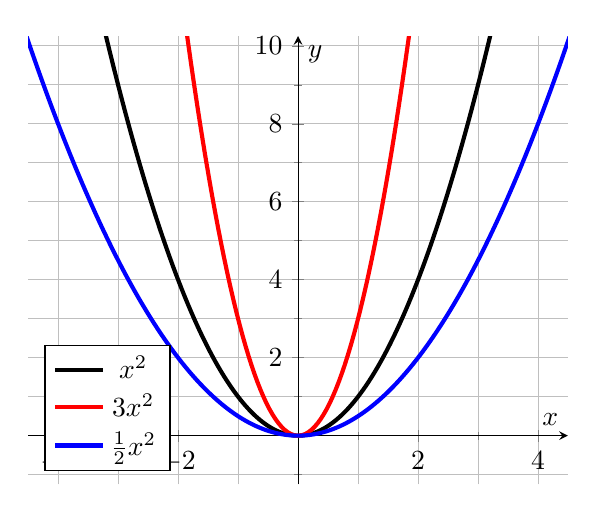
\begin{tikzpicture}
          \begin{axis}[
            axis lines = center,
            grid = both,
            xlabel={$x$},
            ylabel={$y$},
            minor tick num=1,
            legend pos=south west,
            ymax=10.25,
            ymin=-1.25
          ]

            \addplot[black, line width=1.5pt, samples=200]{x^2};
            \addlegendentry{\(x^2\)};

            \addplot[red, line width=1.5pt, samples=200]{3*x^2};
            \addlegendentry{\(3x^2\)};

            \addplot[blue, line width=1.5pt, samples=200]{1/2*x^2};
            \addlegendentry{\(\frac{1}{2}x^2\)};
          \end{axis}
        \end{tikzpicture}
      \end{minipage}

      \item $h$ and $k$ control the $x$ and $y$ coordinate of the vertex, respectively. So, changing the value of $h$ will shift the vertex to the left or the right. A positive value of $h$ will move the vertex to the right while a negative value of $h$ will move the vertex to the left. its important to note that a positive value of $h$ will look negative due to the minus sign in front of the $h$ and a negative value of $h$ will look positive: $a\left(x-\left(-h\right)\right)+k = a\left(x+h\right)+k$. Similar to $h$, changing the value of $k$ will change the vertex's $y$ coordinate. A positive value of $k$ moves the vertex up while a negative value of $k$ moves the vertx down
    \end{enumerate}
  \end{tcolorbox}

  
  \begin{tcolorbox}[breakable, title=GENERAL FUNCTIONS, colframe=black, sharp corners, colback=white, colbacktitle=white, coltitle=black]
    \Large \textbf{Introduction} 
    \newline \normalsize
    In general with most functions there are usually a few things that are of interest to us: \textbf{domain, range, end behavior, and asymptotes}.
    \vspace{0.1in}
    \newline \Large \textbf{Domain and Range}
    \newline \normalsize The domain and range of a function are a special type of set that represent all the possible $x$ and $y$ values a function could take on. When trying to find the domain of a function you must consider what are the possible $x$ value that could be provided to the function in order to get an output. For example, the function $f(x)=x^2$ would have a domain of all real numbers, represented as $\mathbb{R}$\footnote{$\mathbb{R}$ is notation for the set of all real numbers - for more information on special sets and their notations see \href{https://www.mathsisfun.com/sets/number-types.html}{\underline{here}}} or $(-\infty, \infty)$ in interval notation; however, the function $f(x)=\sqrt{x}$ would only have a domain of the positive real numbers (since taking the square root of a negative number would result in a complex number - assume that we are only working in the real numbers), represented as $[0, \infty)$\footnote{This could also be represented as $\mathbb{R}^{\textit{nonneg}}$ or as $\mathbb{R}^{*}$}. As for the range, you must consider the question: for all the possible $x$ values that could be inputted, what are the possible $y$ value outputs? For example, in $f(x)=x^2$ the range would be $[0, \infty)$ because squaring any number makes it positive, thus making it impossible for the squaring function to return a negative number. But, for a function like $f(x)=x^3$ the range would be $(-\infty, \infty)$ since cubing a negative number returns a negative number. The domain and range can also easily be found by looking at the graphs: the graph of $f(x)=\sqrt{x}$ only extends to the right from zero, thus the domain must be $[0, \infty)$ as there are no negative $x$ inputs and the graph of $f(x)=x^2$ only extends upward from zero, so the range must be $[0, \infty)$ as there are no negative $y$ outputs.
  \vspace{0.1in}
  \newline\Large\textbf{End Behavior}
  \newline\normalsize The end behavior of a function analyzes how the outputs behave as the inputs approach extremely Large values (usually positive and negative infinity). The end behavior of a function can be easily identified by looking at a graph or by following a few simple rules. For polynomials look at the leading term (the term with the highest degree exponent), which we will represet as $ax^n$: 
  \begin{enumerate}
    \item If $a$ is positive and $n$ is even then the end behavior of the function is: as $x\to\,\infty, y\to\,\infty$ and as $x\to\,-\infty, y\to\,\infty$ (ex. $f(x)=x^2$)
    \item If $a$ is negative and $n$ is even then the end behavior of the function is: as $x\to\,\infty, y\to\,-\infty$ and as $x\to\,-\infty, y\to\,-\infty$ (ex. $f(x)=-x^2$)
    \item If $a$ is positive and $n$ is odd then the end behavoir of the function is: as $x\to\,\infty, y\to\,\infty$ and as $x\to\,-\infty, y\to\,-\infty$ (ex. $f(x)=x^3$)
    \item If $a$ is negative and $n$ is odd then the end behavoir of the function is: as $x\to\,\infty, y\to\,-\infty$ and as $x\to\,-\infty, y\to\,\infty$ (ex. $f(x)=-x^3$)
  \end{enumerate}
  \vspace{0.1in}
  \Large\textbf{Asymptotes}
  \newline\normalsize Asympototes, both horizontal and vertical, in a function represent $x$ (vertical asympototes) and $y$ (horizontal asympototes) values that a function could not possibly take on. For example, the function $f(x)=\frac{1}{x}$ has a vertical asympototes at $x=0$ and a horizontal asymptotes at $y=0$. To see why this is, first consider if there was no vertical asympotote, then we could have $f(0)=\frac{1}{0}$, but this is division by zero and therefore impossible! So our vertical prevents this error from occuring by stopping $0$ as being a valid input to our function. As for our horizontal asympotote, again consider if there was none - this would mean that at some point in our function $0=\frac{1}{x}$ but if we were to solve for the $x$-coordinate of this point we would find that $0(x)=1 \implies 0=1$!\footnote{Note that the $\implies$ symbol is used to represent 'implies' or 'therefore'} Again, we know that obviously $0 \ne 1$ and so our horizontal asympotote prevents this by stopping $0$ from being a valid output. When it comes to actually finding asympototes, you can begin by looking at a graph of the function and simply just finding which values of $x$ and $y$ the graph will never cross. It's also possible to figure it out simply just by using the function. 
  \vspace{0.05in}
  \newline\large\textbf{Rational Functions}
  \newline\normalsize First, consider the rational function $f(x)=\frac{P(x)}{Q(x)}$. The vertical asympotote will always occur where $Q(x)=0$. As for the horizontal asympotote, there are three different cases:
  \begin{enumerate}
    \item Case 1 ($P(x)$ and $Q(x)$ are of even degree): In the case where both the numerator and denominator's highest degree term are of the same degree then the horizontal asympotote occurs at the ratio of the leading coefficents. For example, in the function $f(x)=\frac{x-2}{8x+30}$, both the numerator and denominator's highest degree term is a first degree term, so the horizontal asympotote occurs at the ratio of the leading coefficents or $y=\frac{1}{8}$
    \item Case 2 ($Q(x)$ is of higher degree than $P(x)$): In the case where the denominator has a term that is higher degree than the numerator, the horizontal asympotote always occurs at $y=0$. For example, $f(x)=\frac{1}{x}$ has a horizontal asympotote at $y=0$
    \item Case 3 ($P(x)$ is of higher degree than $Q(x)$): In this case, there are actually two cases wrapped in 1. In the specific senario where $P(x)$ is a single degree higher than $Q(x)$ the function has no horizontal asympotote, but instead has a slant (or oblique) asympotote which can be found by using polynomial long division to divide $P(x)$ by $Q(x)$ - for an example try graphing the function $f(x)=\frac{x^2+3x+2}{x+3}$. In the other senarios in which $P(x)$ is more than one degree greater than the degree of $Q(x)$, the function has no horizontal asympotote of any kind\footnote{Sometimes it may be possible for these rational functions to have asympototes of higher degrees such as quadratic asympototes, but thats (probably) something you'll never have to worry about}.
  \end{enumerate}
  \vspace{0.05in}
  \large\textbf{Non Rational Functions}
  \newline\normalsize Certain non rational functions can also have horizontal and/or vertical asympototes such as the exponential or logarithmic functions. $f(x)=\textbf{e}^x$ has a horizontal asympotote at $y=0$ while \\ $f(x)=\log\,(x)$ has a vertical asympotote at $x=0$. Again, asympototes here can be deduced by looking at the graph or by looking at the transformations of these functions from the parent function (ex. $f(x)=\textbf{e}^x-2$ would have its horizontal asympototes at $y=-2$ because the graph has been shifted down 2 units)
  \vspace{0.05in}
  \newline\large\textbf{Effects of Asympototes}
  \newline\normalsize Asympototes effect the other two main properties of graphs we discussed, domain, range, and end behavior. When analyzing the domain and range of a graph with an asympotote it often become necessary to split the domain/range into two (or more) seperate sets. For example, $f(x)=\frac{1}{x}$ would have a domain of $(-\infty, 0) \cup (0, \infty)$\footnote{Note that the $\cup$ symbolizes a union and is used to join two sets together}\footnote{As well, note that the asympotote is exclusive in the interval notation representation} and, similarly, a range of $(-\infty, 0) \cup (0, \infty)$. As for its end behavior, pretty logically we can deduce that instead of the graph going off to positive or negative infinity, instead it's going to approach the horizontal asympotote, so for our function $f(x)=\frac{1}{x}$ our end behavoir would look like: as $x\to\,\infty, y\to\,0$ and as $x\to\,-\infty, y\to\,0$.
\end{tcolorbox}
\end{document}
